\documentclass[16pt, letterpaper]{article}
\usepackage{amsmath}
\usepackage{algorithm}
\usepackage{tikz}
\usetikzlibrary{calc}
\newcounter{nodeidx}
\setcounter{nodeidx}{1}
\newcommand{\nodes}[1]{%
    \foreach \num in {#1}{
      \node[minimum size=6mm, draw, rectangle] (\arabic{nodeidx}) at (\arabic{nodeidx},0) {\num};
      \stepcounter{nodeidx}
    }
    % reset counter to re-use command
    \setcounter{nodeidx}{1}
}
\newcommand{\brckt}[4]{% from, to, lvl, text
  \draw (#1.south west) ++($(-.1, -.1) + (-.1*#3, 0)$) -- ++($(0,-.1) + (0,-#3*1.25em)$) -- node [below] {#4} ($(#2.south east) + (.1,-.1) + (.1*#3, 0) + (0,-.1) + (0,-#3*1.25em)$) -- ++($(0,#3*1.25em) + (0,.1)$);%
}

\usepackage[noend]{algpseudocode}
\usepackage{comment}
\title{Gina Cody Scool of Computer Science and Software Engineering \\Concordia University
\\COMP 352: Data Structure and Algorithms
\\Programming Part}
\author{Student: Duc Nguyen}
\date{}
\begin{document}

\begin{titlepage}
\maketitle
\end{titlepage}

\section*{PSEUDO-CODE}
\textbf{Global Variables:}
\begin{itemize}
    \item Stack: a Stack with purpose of keeping track all the passed index in the algorithm. (Empty initialy). 
    \item board: the given array of integer.
\end{itemize}
\begin{algorithm}[H]
\caption{Take input of an integer index, and an  array of integer. Return a boolean value indicates if the game is solvable}
\begin{algorithmic}[1]
\Procedure{checkWinnable(index, board)}{}
\If{$index + 1 = board.length$}\Comment{Terminate case}
\State \Return \textit{true}
\EndIf

\If{$\neg (Stack.search(index)=-1)$}
\State \Return \textit{false}\Comment{Possible redundancy/unsolvable}
\EndIf

\If{$(index < 0) || (index \geq board.length)$}\Comment{Out of bound case}
\State \Return \textit{false}
\EndIf

\State Stack.push(index) \Comment{Valid index, update Stack with new index}
\State\Return \textit{$checkWinnable(index-board[index], board)$
\State $|| checkWinnable(index+board[index], board)$}
\EndProcedure
\end{algorithmic}
\end{algorithm}

\section*{A.}
\subsection*{1. Time complexity}
Since the algorithm uses binary recursion, each half of a call will make \textbf{(n-1)} another recursive calls. There are 2 half of each call, thus it would be \textbf{2n - 2}. However, since the call also calls itself firstly, it becomes \textbf{O(2n-1)}. In addition, the algorithm has to check if the current index was already passed before by \textit{search()} in Stack, results in \textbf{n} of time complexity.
As a result, the time complexity is of \textbf{O(3n-1) = O(n)}.

\subsection*{2. Space complexity}
First of all, the space complexity of the algorithm is of $1 + \log_2 n$ since that is the number of maximum active calls at once. However, in each recursive call, the algorithm also has to keep a Stack to store all the passed index; thus, it takes up to \textbf{n} space. Therefore, the algorithm space complexity is of $O(1 + \log_2 n + n)$ = \textbf{O(n)}.

\section*{B.}
The type of recursion was being used is \textbf{Binary Recursion}. It has no significant change in term of Time complexity, but it has a great impact on reducing space complexity for the algorithm. However, this improvement is covered by the lost of memory for keeping the Stack in this situation.

\section*{C.}
The test logs for the program was generated randomly in order to guarantee the algorithm's efficiency in every possible scenario. 20 test cases are generated, in addition to a few personal test cases (personal configuration).

\section*{D.}
To detect an unsolvable array configuration, it depends mostly on the initial pointer (trigger). Every move after the first trigger should not repeat any of the passed index since it will lead to nowhere. In reality, the player actually can move back to his/her old position and then goes on to another position. However, this is redundancy. In order to win the game in a fastest way, the player should \textbf{only} move pointer to new position. In the other hand, when designing the algorithm, the computer can detect if an array is winnable or not by checking the next possible moves. If the pointer cannot move to anywhere else other than old position or invalid index (out of bound), the configuration is unsolvable.
\\
\begin{tikzpicture}
    \pgftransparencygroup
    \nodes{5, 8, 2 , 3, 1, 5, 0}
    \endpgftransparencygroup
%----End Line 1
    \pgftransparencygroup
    \brckt{1}{1}{0}{index}
    \endpgftransparencygroup
% GIVEN ARRAY
    \pgftransparencygroup
    \brckt{1}{7}{1}{Given Configuration}
    \endpgftransparencygroup
\end{tikzpicture}
\\
\begin{tikzpicture}
    \pgftransparencygroup
    \nodes{0}
    \endpgftransparencygroup
%----End Line 1
    \pgftransparencygroup
    \brckt{1}{1}{0}{Stack}
    \endpgftransparencygroup
\end{tikzpicture}
\Comment{Index was at 0, push(0) to the stack}
\\
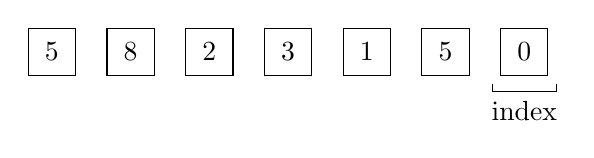
\begin{tikzpicture}
    \pgftransparencygroup
    \nodes{5, 8, 2 , 3, 1, 5, 0}
    \endpgftransparencygroup
%----End Line 1
    \pgftransparencygroup
    \brckt{6}{6}{0}{index}
    \endpgftransparencygroup
\end{tikzpicture}
\Comment{Move index to index 5}
\\
\begin{tikzpicture}
    \pgftransparencygroup
    \nodes{0, $\longleftarrow 5$}
    \endpgftransparencygroup
%----End Line 1
    \pgftransparencygroup
    \brckt{1}{2}{0}{Stack}
    \endpgftransparencygroup
\end{tikzpicture}
\Comment{Index was at 5, push(5) to the stack}
\\
\textbf{At this point, the index (pointer) cannot move 5 steps to the right because it will be out of bound $\longrightarrow$ it moves left}
\\
\\
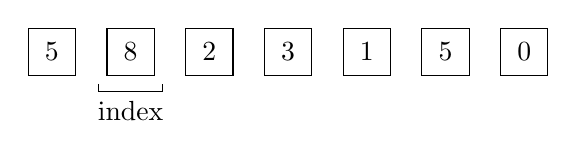
\begin{tikzpicture}
    \pgftransparencygroup
    \nodes{5, 8, 2 , 3, 1, 5, 0}
    \endpgftransparencygroup
%----End Line 1
    \pgftransparencygroup
    \brckt{1}{1}{0}{index}
    \endpgftransparencygroup
\end{tikzpicture}
\Comment{Move index back to 0}
\\
\begin{tikzpicture}
    \pgftransparencygroup
    \nodes{0, 5}
    \endpgftransparencygroup
%----End Line 1
    \pgftransparencygroup
    \brckt{1}{2}{0}{Current stack}
    \endpgftransparencygroup
\end{tikzpicture}
\Comment{Current index is 0; but there was index 0 inside the Stack}
\\
\textbf{Return False, indicates redundancy/unsolvable configuration}

\end{document}
